%Putting here things deleted from other activities, in case we need them later

%% TWO QUESTIONS FROM CONTRAST/PITCH AS ORGINIALLY WRITTEN:
\begin{question}
Consider the first four measures of \textit{Twinkle Twinkle, Little Star}:


\begin{music}
\instrumentnumber{1}            % number of instruments
\setstaffs1{1}              % number of lines per instrument
\generalmeter{\meterfrac{4}{4}}   % time stamp. meterC is 4/4, allabreve is 2/2 or cut time.
\generalsignature{0}            % sets the key. a number greater than 0 is sharp, smaller than 0 is flat
\startextract
% bar 1
  \Notes \Uptext{\metron{\qu}{100}}  \ql j \ql j  \ql n \ql n \en 
\bar % bar 2
  \Notes  \ql o \ql o \hl n  \en 
\bar % bar 3
  \Notes  \ql m \ql m \ql l \ql l  \en 
\bar % bar 4
  \Notes  \ql k \ql k \hl j  \en 
\endextract
\end{music}
  
 Before, you encoded this in the online sequencer. You will need to do it again, since we are going to work some more with it. 
  
   \begin{center}
    \url{https://onlinesequencer.net/}
  \end{center}
  
  Your friends like your encoded passage, but they want it to be ``louder.'' To do this, you can have two notes play at the same time. 
  
 \begin{enumerate}
     \item Add a quarter note on the line directly above each of the first two notes ($D_5$) and play your new composition. Is the first note actually louder like we wanted it to be? Does it sound "nice"?
     \item Move the new notes up to the next white slot ($E_5$). Play it again and compare with what you had before. Does it sound louder or nicer than before?
     \item Keep experimenting by moving the new notes to different positions below the original note and choose a spot that you think sounds ``nice''. How many rows below the original notes are your new notes?
     \item Make copies of all the other notes on the piece. Place each new note the same number of rows below the original ones as you did in the previous step. Does the result sound louder than the original? Is the sound pleasing and does it still sound like \textit{Twinkle Twinkle, Little Star}?
     \item Keep experimenting with the online sequencer. Keep in mind that we want the new piece to
     \begin{itemize}
         \item sound louder (without turning up the volume),
         \item sound like \textit{Twinkle Twinkle, Little Star},
         \item and have a pleasant sound.
     \end{itemize}
 \end{enumerate} 

\end{question}


\begin{instructorNotes}
For this activity, we will need to remind the students (possibly several times) that the 100 cent difference between adjacent keys includes black keys. Thus, for example, $A_3$ and $B_3$ are 200 cents apart, since there's a black key in between them.
\end{instructorNotes}

\begin{question} Look back at the staff that shows \textit{Twinkle Twinkle, Little Star}. What's the difference in cents between each pair of consecutive notes? How can you easily tell that from the online sequencer?

\answerlines

\answerlines

\answerlines


\end{question}

%%%%%%%
%%%%%%%%
%%%%%%%









\begin{center}
$\underset{\raisebox{-.4em}{\text{\small treble clef}}}{\scalebox{1}{\mbox{%
    \smallmusicsize%
    \setclefsymbol1\empty%
    \generalmeter{\empty}%
    \nostartrule%
    \setlines1{0}%
    \setclefsymbol1\trebleclef
    \staffbotmarg0pt%
    \stafftopmarg0pt%
    \startpiece%
    \zstoppiece%
}}}$
\qquad or\qquad
$\underset{\raisebox{-1em}{\text{\small bass clef}}}{\scalebox{1}{\mbox{%
    \smallmusicsize%
    \setclefsymbol1\empty%
    \generalmeter{\empty}%
    \nostartrule%
    \setlines1{0}%
    \setclefsymbol1\bassclef
    \staffbotmarg0pt%
    \stafftopmarg0pt%
    \startpiece%
    \zstoppiece%
}}}$%
\qquad or\qquad
$\underset{\raisebox{-1em}{\text{\small drum clef}}}{
\scalebox{1}{\mbox{%
    \smallmusicsize%
    \setclefsymbol1\empty%
    \generalmeter{\empty}%
    \nostartrule%
    \setlines1{0}%
    \setclefsymbol1\drumclef
    \staffbotmarg0pt%
    \stafftopmarg0pt%
    \startpiece%
    \zstoppiece%
}}}$
\end{center}
and there are others. The first two symbols tell you about what ``pitch'' the notes represent. Today we are more interested in the third. It signifies that we shouldn't worry so much about the pitch, 




\begin{question} %% REWRITE: ORDER OF SHARPS
When writing down sharps, they always come in a specific order. 
\begin{multicols}{4}

\begin{music}
\instrumentnumber{1}            % number of instruments
\setstaffs1{1}              % number of lines per instrument
%generalmeter{\meterfrac{4}{4}}   % time stamp. meterC is 4/4, allabreve is 2/2 or cut time.
\generalsignature{1}           % sets the key. a number greater than 0 is sharp, smaller than 0 is flat
\startextract\endextract
\end{music}

\begin{music}
\instrumentnumber{1}            % number of instruments
\setstaffs1{1}              % number of lines per instrument
%generalmeter{\meterfrac{4}{4}}   % time stamp. meterC is 4/4, allabreve is 2/2 or cut time.
\generalsignature{2}           % sets the key. a number greater than 0 is sharp, smaller than 0 is flat
\startextract\endextract
\end{music}


\begin{music}
\instrumentnumber{1}            % number of instruments
\setstaffs1{1}              % number of lines per instrument
%generalmeter{\meterfrac{4}{4}}   % time stamp. meterC is 4/4, allabreve is 2/2 or cut time.
\generalsignature{3}           % sets the key. a number greater than 0 is sharp, smaller than 0 is flat
\startextract\endextract
\end{music}

\begin{music}
\instrumentnumber{1}            % number of instruments
\setstaffs1{1}              % number of lines per instrument
%generalmeter{\meterfrac{4}{4}}   % time stamp. meterC is 4/4, allabreve is 2/2 or cut time.
\generalsignature{4}           % sets the key. a number greater than 0 is sharp, smaller than 0 is flat
\startextract\endextract
\end{music}
\end{multicols}
The first sharp is an $F$ sharp. To find the order that the sharps are written, start at $F$, and then add $700$ cents, this will give us $C$, which will be our next sharp. Continuing this process gives us the order. 
\begin{enumerate}
\item Draw the ``key signature'' (the sharps on the staff) if there are $5$ sharps.
\item How many sharped notes are there between $C_3$ and $C_4$?
\item Draw the key signature (the sharps on the staff) if there are $6$ sharps.
\end{enumerate}

\end{question}


\begin{question} 
Consider the following excerpt:

\begin{music}
\instrumentnumber{1}            % number of instruments
\setstaffs1{1}              % number of lines per instrument
\generalmeter{\meterfrac{4}{4}}   % time stamp. meterC is 4/4, allabreve is 2/2 or cut time.
\generalsignature{3}            % sets the key. a number greater than 0 is sharp, smaller than 0 is flat
\startextract
% bar 1
  \Notes  \ql e \ql f  \ql g \ql h \en 
\bar % bar 2
  \Notes  \ql i \ql j \ql k \ql l\en 

\endextract
\end{music}
The notes here are:
\[
E, \quad F\sharp, \quad G\sharp,\quad  A,\quad  B,\quad C\sharp,\quad D,\quad E 
\]
What would the notes be named if the key signature was written with:
\begin{enumerate}
\item One flat and two sharps? Check all combinations.
\item What about two flats and and one sharp?  Check all combinations.
\item Three flats?
\item Reflect on your answers above.
\end{enumerate}
\end{question}































\begin{question}%Freq and wavelength
Let's think about how frequency and wavelength are connected. The plot above showed a wave that was changing over time. In this activity we will focus on waves that stay the same size throughout.
\begin{enumerate}
\item Draw a wave with half the \textbf{wavelength} of the wave below:
\begin{center}
    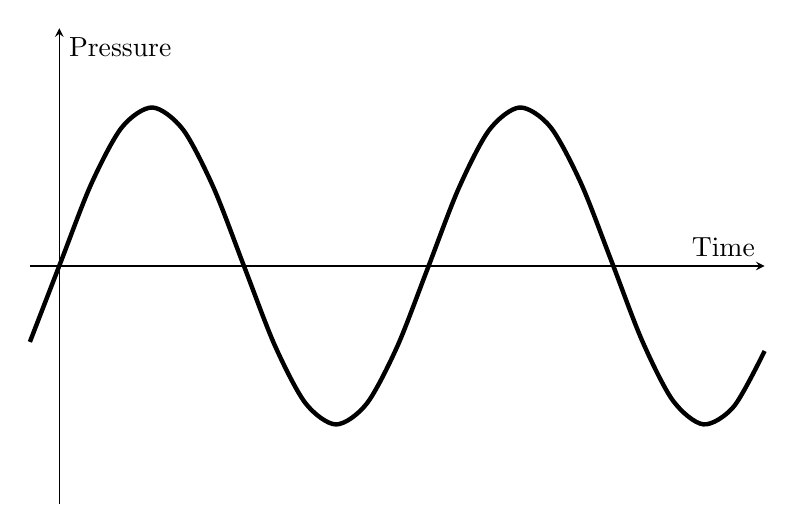
\begin{tikzpicture}
        \begin{axis}[
                xmin=-.5,xmax=12,ymin=-1.5,ymax=1.5,
                axis lines=center,
                ticks=none,  
                width=.9\textwidth,
                height=3in,
                xlabel=Time, ylabel=Pressure,
            clip=false,
              ]       
              \addplot [ultra thick, black,smooth, domain=(-.5:12)] {sin(deg(x))};
            \end{axis}
    \end{tikzpicture}
\end{center}
How is the frequency of the new wave related to the wavelength of the original wave?
\item Draw a wave with three times the \textbf{frequency} of the wave below. 
%Meaning a wave that fits three times as many full waves on a given time interval, than the original wave.
\begin{center}
    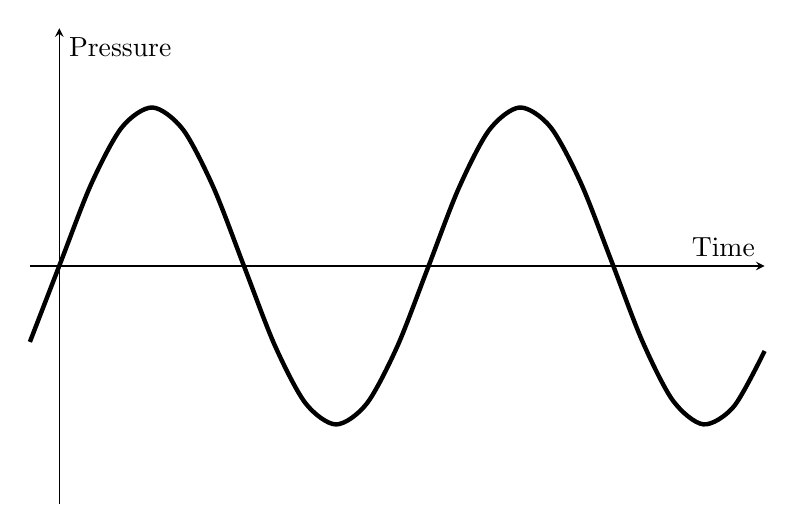
\begin{tikzpicture}
        \begin{axis}[
                xmin=-.5,xmax=12,ymin=-1.5,ymax=1.5,
                axis lines=center,
                ticks=none,  
                width=.9\textwidth,
                height=3in,
                xlabel=Time, ylabel=Pressure,
            clip=false,
              ]       
              \addplot [ultra thick, black,smooth, domain=(-.5:12)] {sin(deg(x))};
            \end{axis}
    \end{tikzpicture}
\end{center}
How is the wavelength of the new wave related to the frequency of the original wave?

\item Describe the relation between frequency and wavelength that you observed in the previous two questions.
\\
\\
\\
\\
\\
\\
\end{enumerate}
\end{question}


\begin{center}
\renewcommand{\arraystretch}{2}
\begin{tabular}{|c|c|c|c|c|c|c|c|c|c|c|c|c|}\hline
Note & $C_3$ & $C_3\sharp$ & $D_3$ & $D_3\sharp$ & $E_3$ & $F_3$ & $F_3\sharp$ & $G_3$ & $G_3\sharp$ & $A_3$ & $B_3\flat$ & $B_3$ \\\hline
Frequency & \hspace{20} & \hspace{20} & \hspace{20} & \hspace{20} & \hspace{20} & \hspace{20} & \hspace{20} & \hspace{20} & \hspace{20} & \hspace{20} & \hspace{20} & \hspace{20} \\\hline
Note & $C_4$ & $C_4\sharp$ & $D_4$ & $D_4\sharp$ & $E_4$ & $F_4$ & $F_4\sharp$ & $G_4$ & $G_4\sharp$ & $A_4$ & $B_4\flat$ & $B_4$ \\\hline
Frequency & \hspace{20} & \hspace{20} & \hspace{20} & \hspace{20} & \hspace{20} & \hspace{20} & \hspace{20} & \hspace{20} & \hspace{20} & \hspace{20} & \hspace{20} & \hspace{20} \\\hline
Note & $C_5$ & $C_5\sharp$ & $D_5$ & $D_5\sharp$ & $E_5$ & $F_5$ & $F_5\sharp$ & $G_5$ & $G_5\sharp$ & $A_5$ & $B_5\flat$ & $B_5$ \\\hline
Frequency & \hspace{20} & \hspace{20} & \hspace{20} & \hspace{20} & \hspace{20} & \hspace{20} & \hspace{20} & \hspace{20} & \hspace{20} & \hspace{20} & \hspace{20} & \hspace{20} \\\hline
Note & $C_6$ & $C_6\sharp$ & $D_6$ & $D_6\sharp$ & $E_6$ & $F_6$ & $F_6\sharp$ & $G_6$ & $G_6\sharp$ & $A_6$ & $B_6\flat$ & $B_6$ \\\hline
Frequency & \hspace{20} & \hspace{20} & \hspace{20} & \hspace{20} & \hspace{20} & \hspace{20} & \hspace{20} & \hspace{20} & \hspace{20} & \hspace{20} & \hspace{20} & \hspace{20} \\\hline
\end{tabular}
\end{center}